\documentclass{article}
\usepackage[utf8]{inputenc}
\usepackage{amsmath}
\usepackage{graphicx}
\usepackage{amsfonts}

\usepackage{mathrsfs} 
\usepackage{float}
\usepackage[ruled,vlined]{algorithm2e}
\usepackage{url}
\newcommand*\mean[1]{\bar{#1}}
\usepackage{amsthm}


\setlength{\parskip}{0.2em}

\title{Métodos numéricos para EDE y aplicación a epidemiología}
\date{}
\begin{document}
\theoremstyle{definition}
\newtheorem{definition}{Definición}[section]
\newtheorem{theorem}{Teorema}
\newtheorem*{definition*}{Definición}
\newtheorem*{theorem*}{Teorema}
\maketitle
\section{Métodos numéricos }
\noindent
Al incluir estocásticidad en el modelamiento de algunos sistemas, surgen ecuaciones diferenciales estocásticas cuya solución exacta sería poco práctico o imposible de encontrar. Por lo tanto, para obtener resultados prácticos se hace necesario desarrollar esquemas de solución que convergen, en cierta manera bien definida, a la solución exacta del problema. En este documento vamos a estudiar algunos métodos de solución numérica de ecuaciones diferenciales estocásticas y vamos a aplicarlos a un caso sencillo de modelación.  \\

\noindent
Vamos a estar interesados en desarrollar soluciones a ecuaciones estocásticas en el sentido de Ito que son de la forma
\begin{equation}
\begin{split}
        dX=a(X)dt+b(X)dW,\\
        X(0)=X_0
\end{split}
\end{equation}
donde $W$ es el movimiento browniano en una dimensión estándar,  $a(X)$ es el termino de drift y $b(X)$ es el coeficiente de difusión, y vamos a exigir que sean lo suficientemente regulares para asegurar la existencia de una solución a esta ecuación diferencial estocástica.\\

\noindent
Existen dos formas de aproximarse al intentar encontrar una solución numérica de este tipo de ecuaciones. La primera consiste en tomar intervalos discretizados de tiempo y usar aproximaciones para los diferenciales involucrados usando una regla de cuadratura para la integral de Ito implícita en la ecuación, y en cada punto de la discretización calcular la solución aproximada. La segunda consiste en intentar resolver la ecuación de Kolmogorov prospectiva o restrospectiva asociada para la obtener la densidad de probabilidad de la solución $X$ en cualquier tiempo. Como esta ecuación es una ecuación diferencial parcial con ciertas condiciones iniciales, se pueden aplicar esquemas en diferencias o elementos finitos para intentar resolverla. Sin embargo, solo se van a tratar algunos de los primeros métodos, puesto que son suficientes en muchos casos y en particular para los que se van a tratar posteriormente.\\

\noindent
Para desarrollar estos métodos, se considera una discretización en el intervalo de tiempo $[0,T]$ dada por $0=\tau_0<\tau_1<\cdots<\tau_n<\cdots \tau_N=T$, usando un tamaño de paso $\Delta=T/N$, siendo también posible escogerlos de manera aleatoria en algunos métodos. No todos los análogos estocásticos de métodos clásicos para soluciónes de ecuaciones diferenciales ordinarias convergen a la solución cuando $\Delta \to 0$.\\

\noindent
Según la aplicación que se requiera, existen diferentes modos de convergencia que pueden definirse 
\theoremstyle{definition}
\begin{definition}
Decimos que una aproximación en tiempo discreto $Y$ a la solución $X$ de una ecuación diferencial estocástica converge fuertemente con orden $\gamma\in(0,\infty]$ si existe una constante $K<\infty$ tal que 
\begin{equation}
    \mathbb{E}(|X_T-Y_N|)\leq K\Delta^{\gamma}
\end{equation}
para todo $\Delta\in(0,1)$
\end{definition}

\begin{definition}
Decimos que una aproximación en tiempo discreto $Y$ a la solución $X$ de una ecuación diferencial estocástica converge debilmente con orden $\beta\in(0,\infty]$ si para todo polinomio $g$ existe una constante $K_g$
 tal que 
 \begin{equation}
    |\mathbb{E}(g(X_T))-\mathbb{E}(g(Y_N))|\leq K_g \Delta^{\beta}
\end{equation}
para todo $\Delta\in(0,1)$. En particular, este tipo de convergencia implica la convergencia de los momentos de $Y$ a los momentos de $X$.
\end{definition}

\noindent
La convergencia fuerte de los métodos se requiere cuando son necesarias simulaciones directas de muestras de los caminos de la solución. La convergencia débil es preferida cuando se requieren otras propiedades de la solución, como promedios o varianzas. En general, los métodos de convergencia débil son más fáciles de implementar que los métodos de convergencia fuerte.\\

\noindent
Para ver de manera heurística de donde surgen los métodos vamos a desarrollar una expansión de Taylor estocástica usando una idea similar a la usada cuando probamos la existencia de soluciones de EDE con iteraciones de Hadamard. En primer lugar, recordemos la formula de Ito en 1-D, que es una expresión modificada de la regla de la cadena para diferenciales estocáticos, si $dX=a(X)dt+b(X)dW$ entonces para una función $f$ dos veces diferenciable se tiene que
\begin{equation}
    df(X)=(f'(X)a(X)+\frac{1}{2}f''(X)b^2(X))dt + f'(X)b(X)dW
\end{equation}
que en forma integral significa 
\begin{equation}
    f(X)=f(X_0)+\int_{t_0}^{t} (f'(X)a(X)+\frac{1}{2}f''(X)b^2(X))ds + \int_{t_0}^{t}f'(X)b(X)dW
\end{equation}
\noindent
Usando la notación compacta de operadores diferenciales, definimos
\begin{equation}
    \mathcal{L}_0=:a(X)\frac{\partial}{\partial X} +\frac{1}{2}b^2(X)\frac{\partial^2}{\partial X^2} 
\end{equation}
\begin{equation}
    \mathcal{L}_1:=b(X)\frac{\partial}{\partial X}
\end{equation}
\noindent
Con los cuales la fórmula de Ito se escribe como 
\begin{equation}
\label{ito:integ}
    f(X)=f(X_0)+\int_{t_0}^{t} \mathcal{L}_0(f(X(s)))ds + \int_{t_0}^{t}\mathcal{L}_1(f(X(s)))dW
\end{equation}

\noindent
En particular, si elegimos $f(X)=a(X)$ y $f(X)=b(X)$ obtendríamos
\begin{equation}
\begin{split}
a(X(t))=a\left(X_0\right)+\int_{t_{0}}^{t} \mathcal{L}_{0} (a(X(s))) d s+\int_{t_{0}}^{t} \mathcal{L}_{1} (a(X(s))) d W\\
b(X(t))=b\left(X_0\right)+\int_{t_{0}}^{t} \mathcal{L}_{0} (b(X(s))) d s+\int_{t_{0}}^{t} \mathcal{L}_{1} (b(X(s))) d W
\end{split}
\end{equation}
luego, insertando estas expresiones en la ecuación estocástica original en su forma integral, obtendríamos
\begin{multline}
X(t)=X_0+\int_{t_{0}}^{t}\left\{a\left(X_0\right)+\int_{t_{0}}^{s_{1}} \mathcal{L}_{0} (a\left(X\left(s_{2}\right)\right))d s_{2}+\int_{t_{0}}^{s_{1}} \mathcal{L}_{1}( a\left(X\left(s_{2}\right)\right)) d W\left(s_{2}\right)\right\} d s_{1}\\ +\int_{t_{0}}^{t}\left\{b\left(X_0\right)+\int_{t_{0}}^{s_{1}} \mathcal{L}_{0}( b\left(X\left(s_{2}\right)\right)) d s_{2}+\int_{t_{0}}^{s_{1}} \mathcal{L}_{1} (b\left(X\left(s_{2}\right)\right)) d W\left(s_{2}\right)\right\} d W\left(s_{1}\right)
\end{multline}
separando todos los términos con integrales dobles en el termino $R$, obtendríamos
\begin{equation}
\label{formulaR}
X(t)=X_0+a\left(X_0\right) \int_{t_{0}}^{t} d s_{1}+b\left(X_0\right) \int_{t_{0}}^{t} d W\left(s_{1}\right)+R,
\end{equation}
donde 
\begin{equation}\begin{aligned}
R = & \int_{t_{0}}^{t} \int_{t_{0}}^{s_{1}} \mathcal{L}_{0} a\left(X\left(s_{2}\right)\right) d s_{2} d s_{1}+\int_{t_{0}}^{t} \int_{t_{0}}^{s_{1}} \mathcal{L}_{1} a\left(X\left(s_{2}\right)\right) d W\left(s_{2}\right) d s_{1} \\
&+\int_{t_{0}}^{t} \int_{t_{0}}^{s_{1}} \mathcal{L}_{0} b\left(X\left(s_{2}\right)\right) d s_{2} d W\left(s_{1}\right)+\int_{t_{0}}^{t} \int_{t_{0}}^{s_{1}} \mathcal{L}_{1} b\left(X\left(s_{2}\right)\right) d W\left(s_{2}\right) d W\left(s_{1}\right)
\end{aligned}\end{equation}
Si queremos aproximar la solución de la ecuación diferencial estocástica que estamos considerando en la discretización temporal propuesta, podríamos ignorar los términos residuales en la fórmula \ref{formulaR} y definir el esquema como
\begin{equation}
    X_{i+1}=X_i+a(X_i)\Delta +b(X_i)\Delta W_i
\end{equation}
donde $\Delta$ es el tamaño de paso en la discretización temporal y $\Delta W_i$ es el cambio en el movimiento browniano que guia el proceso, que puede ser simulado como una variable normalmente distribuida con media $0$ y varianza $\Delta$. Este método es llamado el método de Euler-Maruyama. Es posible probar, no de manera sencilla, que este método tiene orden de convergencia débil $\beta=1$ y orden de convergencia fuerte $\gamma=0.5$, lo que lo convierte en un método poco eficiente para resolver problemas, además tiene pocas propiedades de estabilidad, por lo que ni siquiera está asegurada su convergencia en problemas malcondicionados.\\

\noindent 
Para obtener esquemas con mejores ordenes de convergencia, podríamos repetir este procedimiento iterativamente para obtener integrandos constantes de ordenes superiores.  Por ejemplo, recordando que $\Delta W \approx \sqrt{(\Delta t)}$, el termino de menor orden en los términos residuales $R$ es el último, en particular si elegimos $f=\mathcal{L}_1(b(X))$ en la formula de Ito y lo insertamos en este término obtendríamos
\begin{equation}\begin{aligned}
& \int_{t_{0}}^{t} \int_{t_{0}}^{s_{1}} \mathcal{L}_{1} b\left(X\left(s_{2}\right)\right) d W\left(s_{2}\right) d W\left(s_{1}\right) \\
=& \int_{t_{0}}^{t} \int_{t_{0}}^{s_{1}}\left\{\mathcal{L}_{1} b\left(X_0\right)+\int_{t_{0}}^{s_{2}} \mathcal{L}_{0} \mathcal{L}_{1} b\left(X\left(s_{3}\right)\right) d s_{3}+\int_{t_{0}}^{s_{2}} \mathcal{L}_{1} \mathcal{L}_{1} b\left(X\left(s_{3}\right)\right) d W\left(s_{3}\right)\right\} d W\left(s_{2}\right) d W\left(s_{1}\right)
\end{aligned}\end{equation}
Así que, considerando el termino que es una doble integral, tendríamos 
\begin{equation}\begin{aligned}
X(t)=& X_0+a\left(X_0\right) \int_{t_{0}}^{t} d s_{1}+b\left(X_0\right) \int_{t_{0}}^{t} d W\left(s_{1}\right) \\
&+b\left(X_0\right) b^{\prime}\left(X_{0}\right) \int_{t_{0}}^{t} \int_{t_{0}}^{s_{1}} d W\left(s_{2}\right) d W\left(s_{1}\right)+\tilde{R}
\end{aligned}\end{equation}
donde usamos que $\mathcal{L}_1(b)=bb'$ y denotamos el nuevo conjunto de términos remanentes como $\tilde{R}$. A esta expresión se le denomina expansión de Taylor-Ito para la ecuación diferencial estocástica original. En esta expresión podemos calcular la doble integral como 
\begin{equation}\begin{aligned}
\int_{t_{0}}^{t} \int_{t_{0}}^{s_{1}} d W\left(s_{2}\right) d W\left(s_{1}\right) &=\int_{t_{0}}^{t}\left[W\left(s_{1}\right)-W\left(t_{0}\right)\right] d W\left(s_{1}\right) \\
&=\int_{t_{0}}^{t} W\left(s_{1}\right) d W\left(s_{1}\right)-\int_{t_{0}}^{t} W\left(t_{0}\right) d W\left(s_{1}\right) \\
\end{aligned}\end{equation}
donde aplicando la fórmula de Ito a  $W^2$, $d(W^2)=2W dW+ dt$, obtendríamos 
\begin{equation}\begin{aligned}
\int_{t_{0}}^{t} \int_{t_{0}}^{s_{1}} d W\left(s_{2}\right) d W\left(s_{1}\right)&=\frac{1}{2} \int_{t_{0}}^{t}\left[d W^{2}\left(s_{1}\right)-d t\right]-\int_{t_{0}}^{t} W\left(t_{0}\right) d W\left(s_{1}\right)\\
&=\frac{1}{2}\left[W^{2}(t)-W^{2}\left(t_{0}\right)-\left(t-t_{0}\right)\right]-W\left(t_{0}\right)\left[W(t)-W\left(t_{0}\right)\right]\\
&=\frac{1}{2}\left[W(t)-W\left(t_{0}\right)\right]^{2}-\frac{1}{2}\left(t-t_{0}\right)
\end{aligned}\end{equation}

\noindent
Por lo tanto, tendríamos la siguiente aproximación de Taylor-Ito para $X(t)$,
\begin{equation}\begin{aligned}
    X(t)=X_0 +a(X_0)(t-t_0)+b(X_0)(W(t)-W(t_0))\\+\frac{1}{2}b(X_0)b'(X_0)\left(\left[W(t)-W\left(t_{0}\right)\right]^{2}-\frac{1}{2}\left(t-t_{0}\right)\right)
\end{aligned}\end{equation}
de la cual se puede deducir el llamado esquema de Milstein dado por 
\begin{equation}
    X_{i+1}=X_i+a(X_i)\Delta+b(X_i)\Delta W_i+\frac{1}{2}b(X_i)b'(X_i)\left[(\Delta W_i)^2-\Delta\right]
\end{equation}
el cual tiene mejores propiedades de convergencia que el método de Euler-Maruyama, puesto que su orden de convergencia fuerte es de $\gamma=1$ y de convergencia débil es de $\beta=1$.\\

\noindent
Siguiendo este procedimiento procedimiento de iteración, escogiendo cada vez más términos en la expanción de Taylor-Ito, es posible obtener esquemas con mejores ordenes de convergencia, aunque resultan siendo más complicados puesto que involucran el cálculo de derivadas superiores de los coeficientes de drift y difusión. En general, para obtener esquemas con orden de convergencia $n$, es necesario incluir todos los términos con $n$ integrales en la expansión de Taylor-Ito. \\

\noindent
Para generar esquemas con convergencia débil donde no sea necesario conocer el camino exacto tomado por el movimiento browniano que guia el movimiento es posible sustituir los incrementos en el movimiento browniano por variables aleatorias bi-valuadas con distribución de probabilidad dada por $P(\Delta W_i=\pm\sqrt{\Delta})=0.5$.\\

\noindent
Con el fin de ilustrar de manera práctica estos métodos, vamos a implementarlos para resolver la ecuación diferencial estocástica
\begin{equation}
    dX=\mu Xdt+\sigma X dW
\end{equation}
con condición inicial $X(0)=X_0$
\nocite{*}
de la cual conocemos una solución exacta dada por 
\begin{equation}
    X(t)=X_0 e^{(\mu-\frac{1}{2}\sigma^2)t-\sigma W}
\end{equation}
que podemos comprobar fácimente con la formula de Ito. En esta simulación escogemos $\mu=2$,$\sigma=1$y $X_0=1$ y simulamos el movimiento browniano escogiendo los incrementos de una variable aleatoria normalmente distribuida con media cero y varianza $\Delta$. En la siguiente figura se muestra la solución exacta comparada con las obtenida numéricamente por ambos métodos con uno de los caminos brownianos usados.
\begin{figure}[H]
    \centering
    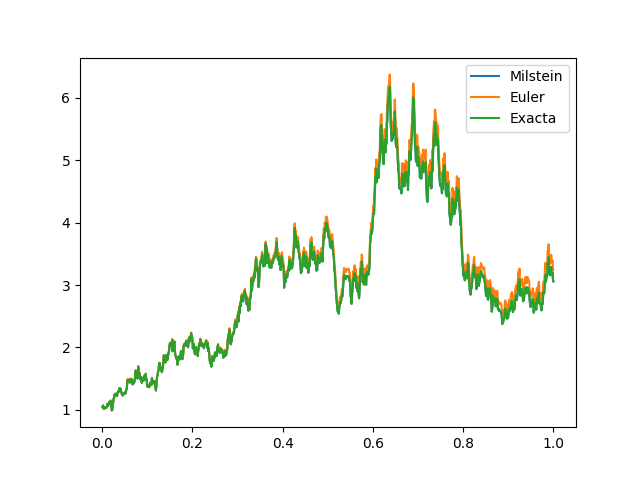
\includegraphics[width=\textwidth]{browniano.png}
    \caption{Decrecimiento del error para los métodos de Euler y Milstein}
    \label{fig:my_label}
\end{figure}
\noindent
Para observar la velocidad de convergencia, calculamos los errores débiles y fuertes y los graficamos a continuación 
\begin{figure}[H]
    \centering
    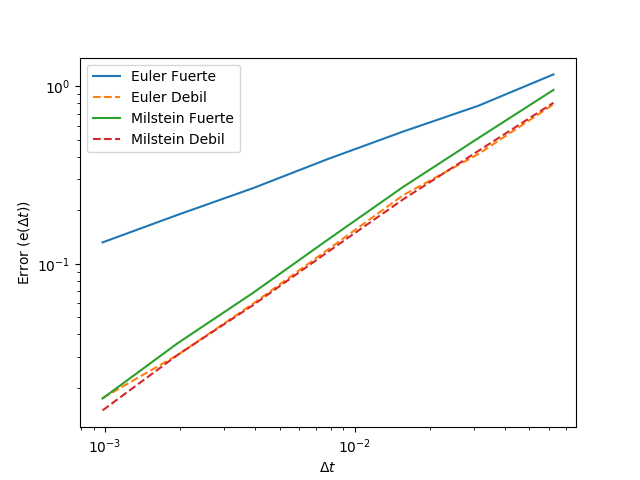
\includegraphics[width=\textwidth]{Convergencia.png}
    \caption{Decrecimiento del error para los métodos de Euler y Milstein}
    \label{fig:my_label}
\end{figure}
donde observamos que se tiene convergencia cuando $\Delta \to 0$ en ambos sentidos, y además el método de Milstein lo hace más rápido en el sentido fuerte.\\

\noindent
Existen modificaciones de estos métodos que además de mejorar el orden de convergencia, mejoran también su eficiencia cuando se enfrentan con problemas mal condicionados, por ejemplo, existen versiones implícitas del método de Euler-Maruyama que muestra mejores propiedades de estabilidad.

\section{Aplicaciones}
Para realizar el modelamiento de sistemas reales en cuya dinámica se  quieran incluir factores estocásticos se procede de manera similar a como se haría con sistemas deterministas. El procedimiento general es encontrar como varia la densidad de probabilidad que describe los estados y asociarla a una ecuación prospectiva de Kolmogorov que cumpliría la densidad de probabilidad de una ecuación diferencial estocásticas.\\

\noindent
Para ilustrar este procedimiento, examinemos un modelo epidemiológico compartimental de carácter estocástico. Vamos a trabajar sobre el modelo SIS para una población, que modela una enfermedad contagiosa que adquieren los individuos sanos (S), pasando a estar en el conjunto de los infectados (I), para después recuperarse y volver a estar sanos. No vamos a considerar nacimientos ni muertes debidas a esta enfermedad, ni a ninguna otra causa, por lo que el tamaño de la población permanece constante. \\

\noindent
El tamaño de la población de infectados en un tiempo $t$ se denota por $I(t)$, y el de la población sana por $S(t)$. Modelamos el proceso de infección con tasas de conversión de personas entre estos estados, $m_{12}$ es la tasa a la cual se infectan personas y $m_{21}$ es la tasa a la que se recuperan. Esta interacción entre las poblaciones se presenta en el siguiente diagrama 
\begin{figure}[H]
    \centering
    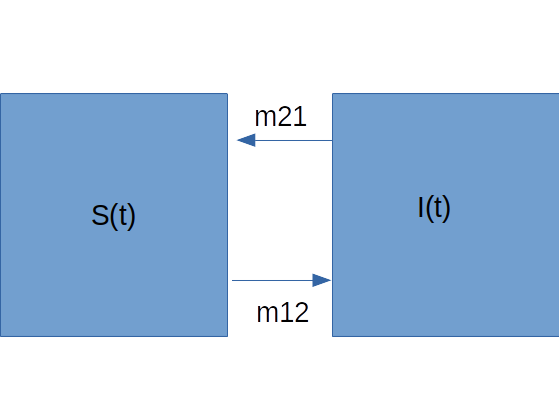
\includegraphics[width=0.65\textwidth]{malf.png}
    \caption{Modelo SIS}
    \label{fig:my_label}
\end{figure}

\noindent
Al estado del sistema lo denotamos por $\mathbf{x}=[S,I]$.
En un intervalo de tiempo $\Delta t$ lo suficientemente pequeño hay 3 posibilidades de que suceda algo, cada una con su respectiva probabilidad, información que podemos resumir en la siguiente tabla
\begin{equation}\begin{array}{ll}
\hline \text { Cambio } & \text { Probabilidad } \\
\hline \Delta \mathbf{x}_{1}=[-1,1]^{T} & p_{1}=m_{12} S \Delta t \\
\Delta \mathbf{x}_{2}=[1,-1]^{T} & p_{2}=m_{21} I \Delta t \\
\Delta \mathbf{x}_{3}=[0,0]^{T} & p_{3}=1-p_1-p_2 \\
\hline
\end{array}\end{equation}
Denotamos por $p(t,S,I)$ la probabilidad de que el sistema tenga $S$ personas sanas e $I$ enfermas en el tiempo $t$. Luego de un tiempo $\Delta t$, la probabilidad de estar en el mismo estado sería,
\begin{equation}
\begin{aligned}
    p(t+\Delta t,S,I)=p(t,S,I)&+\Delta t (p(t,S+1,I-1)m_{12}(t,S+1,I-1))\\
    &+\Delta t (p(t,S-1,I+1)m_{21}(t,S-1,I+1))\\
    &-\Delta t (p(x,S,I)(m_{21}(t,S,I)+m_{12}(t,S,I)).
\end{aligned}
\end{equation}
\noindent
En esta expresión, el primer termino está asociado a la contribución de probabilidad de que ya se esté en el estado $(S,I)$ y en el intervalo de tiempo no pase nada, el segundo termino es la contribución a la probabilidad que se porque existe la posibilidad de que el estado $(S+1,I-1)$ pase al estado $(S,I)$ cuando enferma una persona, el tercer termino es similar pero en el caso contrario cuando se pasa del estado $(S-1,I+1)$ al estado $(S,I)$, y finalmente el cuarto termino es la contribución que se da cuando ya se está en el estado $(S,I)$ y sucede alguna transición entre las poblaciones.\\

\noindent
En un intervalo de tiempo pequeño, podemos aproximar el segundo y tercer termino mediante su serie de Taylor en segundo grado al rededor de $(t,SI,)$, así
\begin{equation}
\begin{aligned}
p(t,S+1,I-1)m_{12}(t,S+1,I-1)
&\approx p m_{12}+\frac{\partial\left(p m_{12}\right)}{\partial S} -\frac{\partial\left(p m_{12}\right)}{\partial I} \\
+&\frac{1}{2} \left[\frac{\partial^2(p m_{12})}{\partial S^2}-2\frac{\partial^2(p m_{12})}{\partial S \partial I}+\frac{\partial^2(p m_{12})}{\partial I^2}\right]
\end{aligned}
\end{equation}
\begin{equation}
\begin{aligned}
p(t,S+1,I-1)m_{21}(t,S+1,I-1)
&\approx p m_{21}-\frac{\partial\left(p m_{21}\right)}{\partial S} +\frac{\partial\left(p m_{21}\right)}{\partial I} \\
+&\frac{1}{2} \left[\frac{\partial^2(p m_{21})}{\partial S^2}-2\frac{\partial^2(p m_{21})}{\partial S \partial I}+\frac{\partial^2(p m_{21})}{\partial I^2}\right]
\end{aligned}
\end{equation}
Por lo que, reorganizando los términos en la expresión 23 y tomando el límite $\Delta \to 0$, obtendríamos que la función de probabilidad satisface la ecuación diferencial 
\begin{equation}
\begin{aligned}
&\frac{\partial p}{\partial t}=\frac{\partial}{\partial S}(m_{12}-m_{21})p+\frac{\partial}{\partial I}(m_{21}-m_{12})p\\
&+\frac{1}{2} \left[\frac{\partial^2(p m_{21})}{\partial S^2}-2\frac{\partial^2(p m_{21})}{\partial S \partial I}+\frac{\partial^2(p m_{21})}{\partial I^2}\right]\\
&+\frac{1}{2} \left[\frac{\partial^2(p m_{12})}{\partial S^2}-2\frac{\partial^2(p m_{12})}{\partial S \partial I}+\frac{\partial^2(p m_{12})}{\partial I^2}\right]
\end{aligned}
\end{equation}
\noindent
Que es una ecuación de Kolmogorov prospectiva(Fokker-Planck). Luego, cualquier función de probabilidad que satisfaga esta ecuación, será la densidad de una variable aleatoria $X=(S,I)$ que cumpla las ecuación diferenciales estocásticas acopladas
\begin{equation}
    \begin{aligned}
    dS=(m_{21}I-m_{12}S)dt+\sqrt{\frac{m_{12}S+m_{21}I}{2}}(dW_1-dW_2)\\
    dI=(m_{12}S-m_{21}I)dt+\sqrt{\frac{m_{12}S+m_{21}I}{2}}(-dW_1+dW_2)
    \end{aligned}
\end{equation}
donde $W_1$ y $W_2$ son dos movimientos brownianos independientes que están asociados a los procesos estocásticos que se presentan en cada sub-población.\\

\noindent
Una vez obtenidas las ecuaciones que modelan el sistema, es fácil implementar métodos numéricos como los vistos en la sección anterior para resolverlo dadas ciertas condiciones iniciales. A partir de este modelo, es posible calcular cantidades como los valores esperados de la cantidad de gente sana o infectada.\\

\noindent
La elección de los parámetros con los que se describe el sistema, como las tasas de infección o recuperación, es un gran problema cuando se intentan usar este tipo de modelos para describir situaciones de la vida real. Una alternativa es usar muestreos de datos en tiempo real para estimar estos parámetros y usar el modelo para realizar predicciones. Evidentemente este modelo tan simplificado solo sirve como ejemplo y no proporcionaría resultados precisos en una situación real.\\

\noindent 
Vamos a resolver estas ecuaciones numéricamente con los siguientes parámetros 
\begin{equation*}
\begin{split}
        m_{12}&=\alpha \frac{I}{I+S}\\
        m_{21}&=\gamma
\end{split}
\end{equation*}
con $\alpha=0.04$, $\gamma=0.01$, y los valores iniciales $S(0)=950$ y $I(0)=50$, y vamos a calcular los valores esperados de número de personas sanas y contagiadas hasta el tiempo $t=100$. Para resolverlo se usó la discretización propuesta por el método de Euler-Maruyama usado anteriormente. A continuación se muestra el promedio obtenido de la solución a lo largo de 20000 trayectorias brownianas, y en la gráfica se muestra la solución obtenida con una de ellas.
\begin{figure}[H]
    \centering
    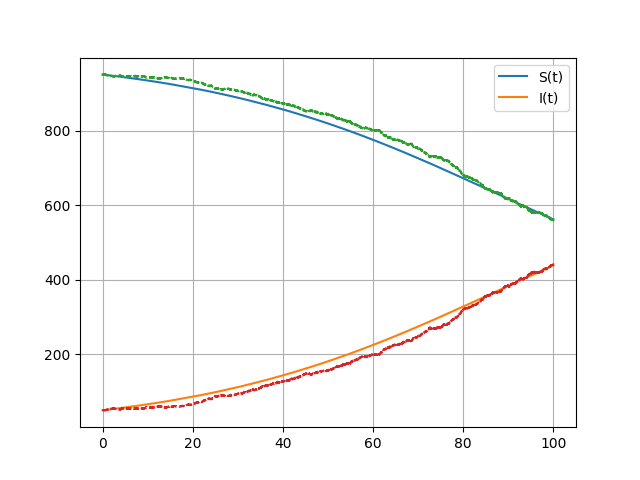
\includegraphics[width=0.5\textwidth]{SimulacionEpide.png}
    \caption{Comportamiento estocástico del modelo SIS}
    \label{fig:my_label}
\end{figure}
que concuerda con los resultados que muestra el libro.


\bibliography{references}
\bibliographystyle{unsrt}
\end{document}
